\subsubsection{01.12.2015}
\textit{\textbf{Time frame:}} 16:00-22:00 \newline
The winch was installed onto the robot. The 8mm axis will be connected with the winch. It will keep the coils for rope. There were drilled all the needed holes for fixing coils on the axis (figure \ref{Winch1.11}, \ref{Winch1.12}). \newline
The gripper was reassembled with the tetrix tube. For powering the gripper it was installed a standard DC motor with gear ratio 2:1.

\begin{figure}[H]
	\begin{minipage}[h]{0.58\linewidth}
		\center{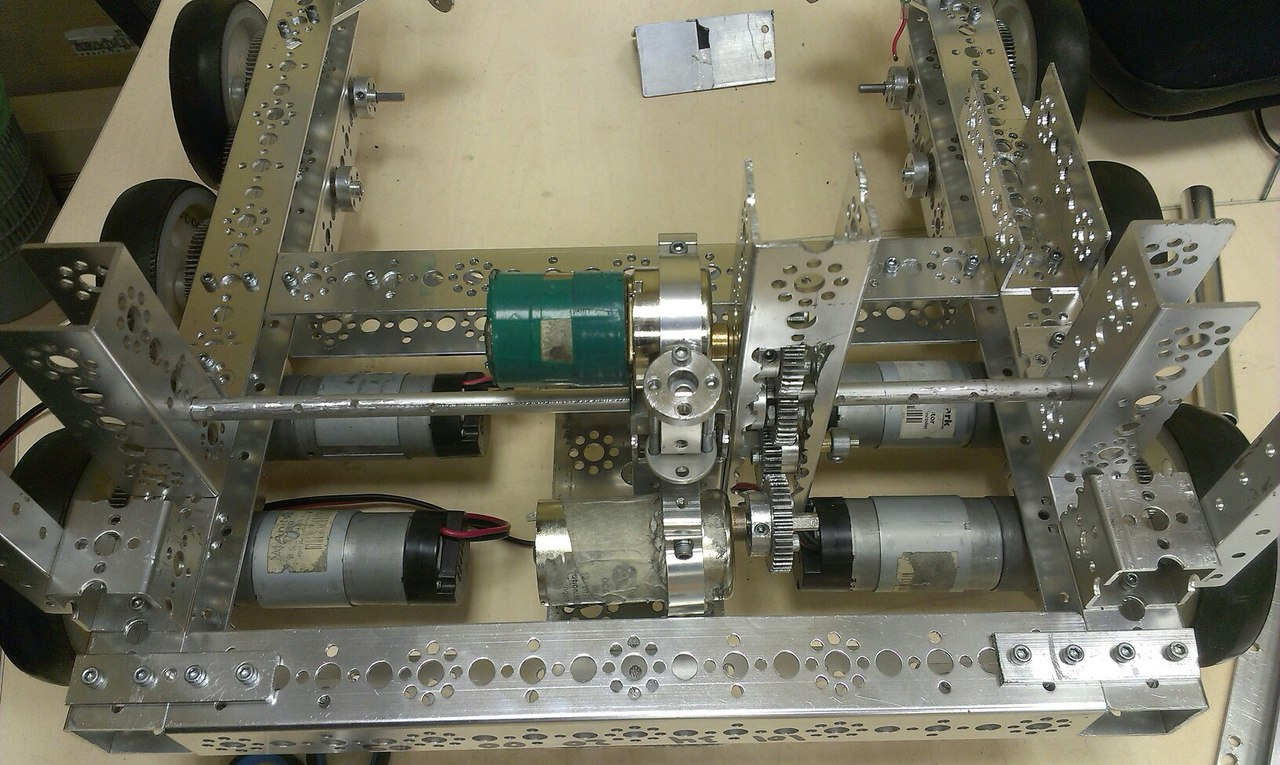
\includegraphics[scale=0.2]{3Engineering/5Team_meetings/days_of_meetings/2015.12.01/images/01}}
		\caption{Winch installed onto the carriage}
		\label{Winch1.11}
	\end{minipage}
	\hfill
	\begin{minipage}[h]{0.37\linewidth}
		\center{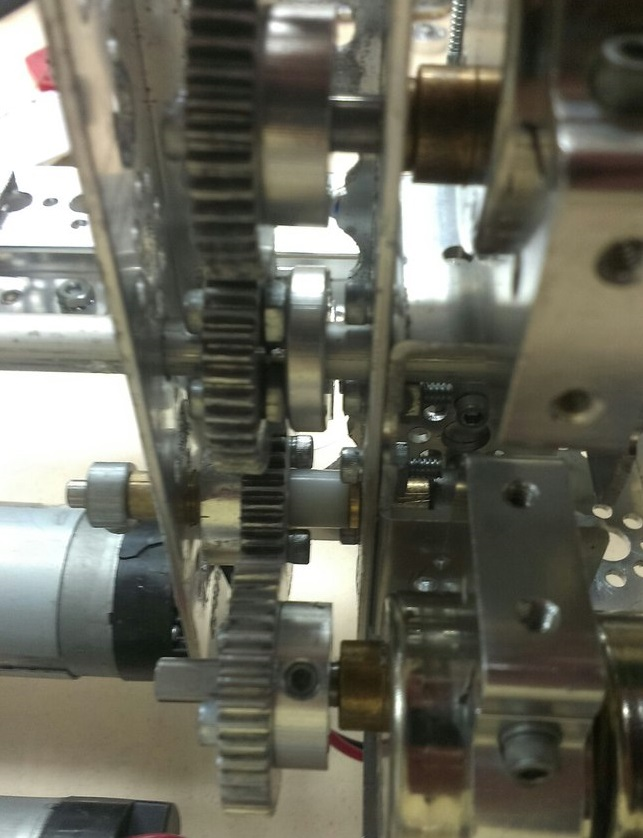
\includegraphics[scale=0.22]{3Engineering/5Team_meetings/days_of_meetings/2015.12.01/images/02}}
		\caption{The construction of the winch}
		\label{Winch1.12}
	\end{minipage}
\end{figure}
